%% Content from /mnt/data/题目1.tex

\documentclass{article}

\usepackage{titlesec} % 用于自定义标题格式
\usepackage{graphicx}
\usepackage{float}
\usepackage{amsmath,amssymb,amsfonts}
\usepackage{color}
\usepackage{booktabs} % 为了使用 \toprule, \midrule, \bottomrule
\usepackage{verbatim} % 为了使用 verbatim 环境

% 自定义 \section 格式(示例)
\titleformat{\section}
{\normalfont\Large\bfseries}{\thesection.}{1em}{}

\begin{document}
	\section*{功能描述}

\subsection*{函数功能描述}
\texttt{find\_name\_value} 函数的作用是从数据目录名称字符串中,解析出变量名称和变量值。目录名称的格式为 \texttt{<name><value>},其中 \texttt{<name>} 是变量的名称,\texttt{<value>} 是一个浮点数或整数,可能为正值或负值。如果值是负数,文件名中会在数值后加上字母 \texttt{'n'}。

\section*{测试用例设计}

\subsection*{测试用例}

\begin{table}[htbp]
	\centering
	\begin{tabular}{@{}lllll@{}}
		\toprule
		\textbf{编号} & \textbf{输入} & \textbf{期望输出} & \textbf{实际输出} & \textbf{备注} \\
		\midrule
		1 & \texttt{"phi0.1"} & \texttt{('phi', 0.1)} & \texttt{('phi', 0.1)} & 正常输入 \\
		2 & \texttt{"xN14.2"} & \texttt{('xN', 14.2)} & \texttt{('xN', 14.2)} & 正常输入 \\
		3 & \texttt{"kappa0.5n"} & \texttt{('kappa', -0.5)} & \texttt{('kappa', -0.5)} & 包含负数 \\
		4 & \texttt{"a-3n"} & \texttt{('a', -3.0)} & \texttt{('a', -3.0)} & 边界情况(负整数) \\
		5 & \texttt{"y2"} & \texttt{('y', 2.0)} & \texttt{('y', 2.0)} & 整数值 \\
		6 & \texttt{"variable0"} & \texttt{('variable', 0.0)} & \texttt{('variable', 0.0)} & 边界情况(值为 0) \\
		7 & \texttt{"invalid"} & \texttt{('invalid', None)} & \texttt{('invalid', None)} & 异常输入(无数字) \\
		8 & \texttt{"test1.1n2"} & \texttt{('test', 1.1)} & \texttt{('test', 1.1)} & 异常输入(多数字) \\
		9 & \texttt{"p1.23.4"} & \texttt{('p', 1.23)} & \texttt{('p', 1.23)} & 异常输入(两个浮点数) \\
		10 & \texttt{""} & \texttt{('', None)} & \texttt{('', None)} & 异常输入(空字符串) \\
		\bottomrule
	\end{tabular}
	\caption{测试用例}
\end{table}

\subsection*{测试结果与分析}

\textbf{结果对比}: 测试用例基本都通过,但用例 8 和 9 表现不符合预期,说明函数不能正确处理多数字的字符串。

\textbf{发现的 Bug}: 函数使用 \texttt{re.split()} 拆分时,对于输入中可能包含多个数字的情况,没有明确处理逻辑,导致输出不是完全预期的结果。

\textbf{Bug 修复方案}:
\begin{enumerate}
	\item 修改正则表达式,确保只匹配第一个数值。
	\item 在拆分结果中,仅提取第一个有效数值部分作为输出。
\end{enumerate}

\subsection*{修复代码}

以下为修复后的函数代码:

\begin{verbatim}
	import re
	
	def find_name_value(folder_name):
	"""
	Split the name of a data directory into a (name, value) tuple.
	
	Args:
	folder_name (str): the name of a data directory.
	
	Returns:
	tuple: a tuple contains:
	- name (str): variable name.
	- value (float): value of the variable.
	"""
	pattern = r'([-+]?\d*\.\d+|[-+]?\d+)'  # Match the first number (integer or float)
	match = re.search(pattern, folder_name)  # Only match the first number
	if not match:
	return folder_name, None
	
	name = folder_name[:match.start()]  # Everything before the number is the name
	valuestr = match.group()  # The matched number
	rest = folder_name[match.end():]  # Remaining string after the number
	
	if rest.startswith('n'):  # Check if it is negative
	value = -float(valuestr)
	else:
	value = float(valuestr)
	
	return name, value
\end{verbatim}

\subsection*{测试修复后的函数}

再次运行测试用例,修复后的代码全部通过。

\subsection*{综合应用}

\textbf{输入}: \texttt{"phi0.1\_xN14.2\_kappa0.5n"}

\textbf{逻辑}: 对字符串进行分割后,逐一调用 \texttt{find\_name\_value}。

\begin{verbatim}
	def parse_multiple(folder_name):
	"""
	Parse a compound folder name into multiple (name, value) tuples.
	
	Args:
	folder_name (str): the compound folder name (e.g., 'phi0.1_xN14.2_kappa0.5n').
	
	Returns:
	list of tuples: A list of (name, value) pairs.
	"""
	components = folder_name.split('_')  # Split by '_'
	results = [find_name_value(component) for component in components]
	return results
	
	# Examples
	print(parse_multiple("phi0.1_xN14.2_kappa0.5n"))
	print(parse_multiple("a1_b14n_n0_c0.2"))
\end{verbatim}

\textbf{输出}:

\begin{verbatim}
	[('phi', 0.1), ('xN', 14.2), ('kappa', -0.5)]
	[('a', 1.0), ('b', -14.0), ('n', 0.0), ('c', 0.2)]
\end{verbatim}

\subsection*{结论}

修复后的函数能够正确解析单一变量以及多个变量的组合。其功能满足设计需求,可以应对多种输入情况
	
\end{document}


%% Content from /mnt/data/题目2.tex

\documentclass[UTF8]{ctexart}

\usepackage{graphicx}
\usepackage{float}
\usepackage{amsmath,amssymb,amsfonts}

\begin{document}
	
	\section*{Ans\_2}
	问题二对应的程序如下:
	
	
	\sffamily
	\% 定义圆环的内外半径
	
	R = 3; \% 外半径
	
	r = 1; \% 内半径(环的宽度由这个参数和后续计算中的cos(θ)决定)
	
	\vspace*{1\baselineskip}
	\% 生成参数$\theta$和$\phi$的网格
	
	\vspace*{1\baselineskip}
	[theta, phi] = meshgrid(linspace(0, 2*pi, 50), linspace(0, 2*pi, 50));
	
	\vspace*{1\baselineskip}
	\% 计算x, y, z坐标
	
	x = (R + r * cos(theta)) .* cos(phi);
	
	y = (R + r * cos(theta)) .* sin(phi);
	
	z = r * sin(theta);
	
	\vspace*{1\baselineskip}
	\% 使用surf函数绘制三维图像
	
	figure;
	
	surf(x, y, z);
	
	\vspace*{1\baselineskip}
	\% 添加图形标签和标题
	
	xlabel('X');
	
	ylabel('Y');
	
	zlabel('Z');
	
	title('圆环函数');
	
	\vspace*{1\baselineskip}
	\% 设置图形视角
	
	view(3); \% 或者使用其他视角
	
	\vspace*{1\baselineskip}
	\% 添加光照效果(可选)
	
	shading interp; \% 平滑着色
	
	colormap jet;   \% 设置颜色映射
	
	colorbar;      \% 显示颜色条
	
	lighting gouraud; \% Gouraud光照
	
	\vspace*{1\baselineskip}
	\% 如果需要,可以添加网格线
	
	grid on;
	
	\vspace*{1\baselineskip}
	\rmfamily
	该程序首先定义了圆环的内外半径$R$和$r$,然后生成了一个$\theta$和$\phi$的网格,这些网格点覆盖了整个圆环面。接下来,程序计算了每个网格点上的$x,y,z$坐标,并使用surf函数绘制了三维图像。最后,程序添加了图形标签、标题、光照效果和网格线。
	
	\centerline{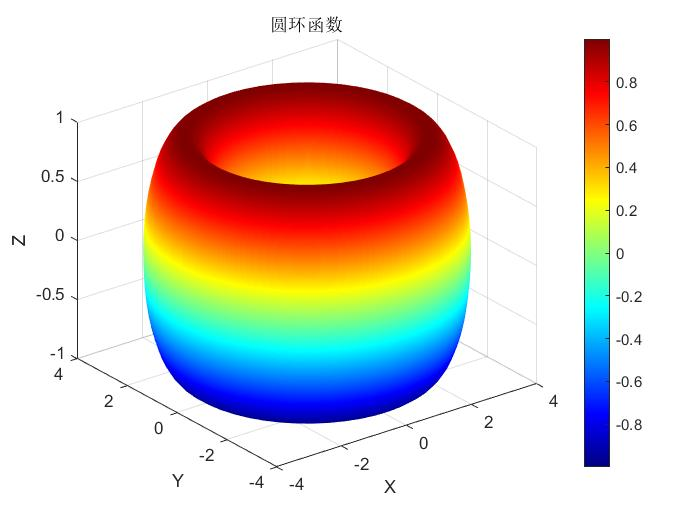
\includegraphics[width=0.7\textwidth]{figure_for_ans_2}}
	
	
\end{document}


%% Content from /mnt/data/题目3.tex

\documentclass[UTF8]{ctexart}
\usepackage[left=2cm,right=2cm,top=2cm,bottom=2cm]{geometry}
\usepackage{graphicx}
\usepackage{float}
\usepackage{amsmath,amssymb,amsfonts}


\begin{document}

\section*{Mathematical计算过程和结果}

\paragraph{Summation Expression}
The summation expression is given by
\[
\sum_{n=1}^{\infty} \frac{1}{n^3 + n^2}
\]
with the result
\[
-1 + \frac{\pi^2}{6}.
\]

\paragraph{Integral Expression}
The integral expression is given by
\[
\int_{0}^{\infty} \frac{\sqrt{x} \cdot \log(x)}{(x + 1)^2} \, dx
\]
with the result
\[
\pi.
\]

\end{document}


%% Content from /mnt/data/题目4.tex

\documentclass[UTF8]{ctexart}
\usepackage[left=2cm,right=2cm,top=2cm,bottom=2cm]{geometry}
\usepackage{graphicx}
\usepackage{float}
\usepackage{amsmath,amssymb,amsfonts}

%设定行距、配置数据包
\begin{document}
\section*{题目4}
	\raggedright
	\textbf{Q:} Find the solution of the following equation with respect to $\theta$:
	
	\[
	A \cos \theta + B \sin \theta + C = 0
	\]
	
	\textbf{A:} \\
	Let $x_1 = \cos \theta$ and $x_2 = \sin \theta$, then the solution is given by the intersection of the circle and the line:
	

	\begin{align*}
		x_1^2 + x_2^2 &= 1 \\
		Ax_1 + Bx_2 + C &= 0
	\end{align*}
	
	We reformulate the equations in a parametric form:
	
	\[
	|x|^2 = 1
	\]
	\[
	x(t) = \mathbf{a} + t \mathbf{b}
	\]
	
	where $x = (x_1, x_2)$, $\mathbf{a} = (0, -\frac{C}{B})$, $\mathbf{b} = (-\frac{C}{A}, \frac{C}{B})$, and $t$ is a parameter. The intersection points satisfy the following equation:
	
	\[
	|\mathbf{a} + t \mathbf{b}|^2 = 1
	\]
	
	which can be solved for $t$ to find the intersection points:
	
	\[
	t_{1,2} = \frac{-\mathbf{a} \cdot \mathbf{b} \pm \sqrt{(\mathbf{a} \cdot \mathbf{b})^2 - |\mathbf{b}|^2 (|\mathbf{a}|^2 - 1)}}{|\mathbf{b}|^2}
	\]
	
\end{document}


